
\addcontentsline{toc}{section}{\uppercase{Introduction}S}
\section*{Introduction}



Активное распространение роботов после середины 20 века привело к автоматизации почти всех аспектов производственных процессов, включая сборку, сварку, покраску, контроль качества и упаковку. Это также оказало значительное влияние на логистику, складское хозяйство
и дистрибуцию, где роботизированные системы используются для сортировки, перемещения и
хранения товаров. Прогресс в области механики, электроники и цифровых устройств, привел к
созданию инновационных устройств. 
Использование существующих универсальных мини роботов манипуляторов является эффективным и рациональным решением, ввиду их небольшого размера и параметров соответствующих для работы с мелкими деталями и конструкциями. Однако несмотря на преимущества мини роботов манипуляторов, они обладают недостатками. Главным недостатком является опасность работы роботов совместно с людьми. Для организации работы данных роботов необходимо создавать специальные закрытые рабочие зоны, для минимизации возможного риска, а работа совместно с человеком представляется невозможной.  Мини робот не может стать коллаборативным если ограничить мощность или силу для каждого звена. Для того что бы робот являлся коллаборативным необходимо производить изменения в конструкции самого робота. Размер мини роботов манипуляторов создает ограничения
для всех элементов системы, установка датчиков момента силы не является лучшим решением,
так как занимают дополнительное пространство в каждом звене робота и усложняют конструкцию мини робота. 

Наиболее подходящий тип электродвигателя является бесщеточный двигатель постоянного тока, для обеспечения всеми особенностями коллаборативного робота, тип BLDC двигателя Gimbal motors наиболее подходящим. 

Целью работы является: Демонстрация возможности использования двигателя типа от карданных камер (gimbal motors) для создания системы управления коллаборативного мини робота манипулятора с учетом упрощения их механической конструкции.

Работа содержит 5 разделов. В первом разделе производится анализ мини роботов манипуляторов, которые доступны на рынке и их характеристики. Исследуются различные варианты двигателей и производится выбор, разработка функций и технических параметров для системы управления мини роботом.  Во втором разделе производится разработка структурной схемы на основе иерархической парадигмы управления роботом, а также алгоритма её описания для системы управления мини роботом. В третьем разделе производится разработка функциональной схемы и описание и назначения ее элементов. В четвертом разделе производится разработка принципиальной схемы с ее описанием, расчет элементов схемы. В пятой части производится разработка алгоритмов и программная реализация на микроконтроллере. 

\section{ Actuality of developing a control system for a mini-robot}


%%%%%%%%%%%%%%%%%%%%%%%%%%%%%%%%%%%%%%%%%%%%%%%%%%%%%%%%%%%%%%%%%%%%%%%%%%%%%%%%%%%%%%%
\subsection{Purpose and classification of robot arms} 
Industrial robots, and in particular manipulating robots, 
have a wide range of applications in a variety of sectors and 
offer many advantages, including increased productivity, accuracy 
and safety. Certain types of robots may be better suited to a particular 
application than others.
\begin{itemize}[itemsep=0pt]
    \item Welding
    \item Material Handling
    \item Assembly
    \item Painting and Coating
    \item Packaging
    \item Inspection and Quality Control
    \item Machine Tending
    \item Surgery and Medical Procedures
    \item Research and Development
    \item Education and Training
    \item Cleaning and Maintenance
\end{itemize}

\begin{figure}[H]
	\centering
	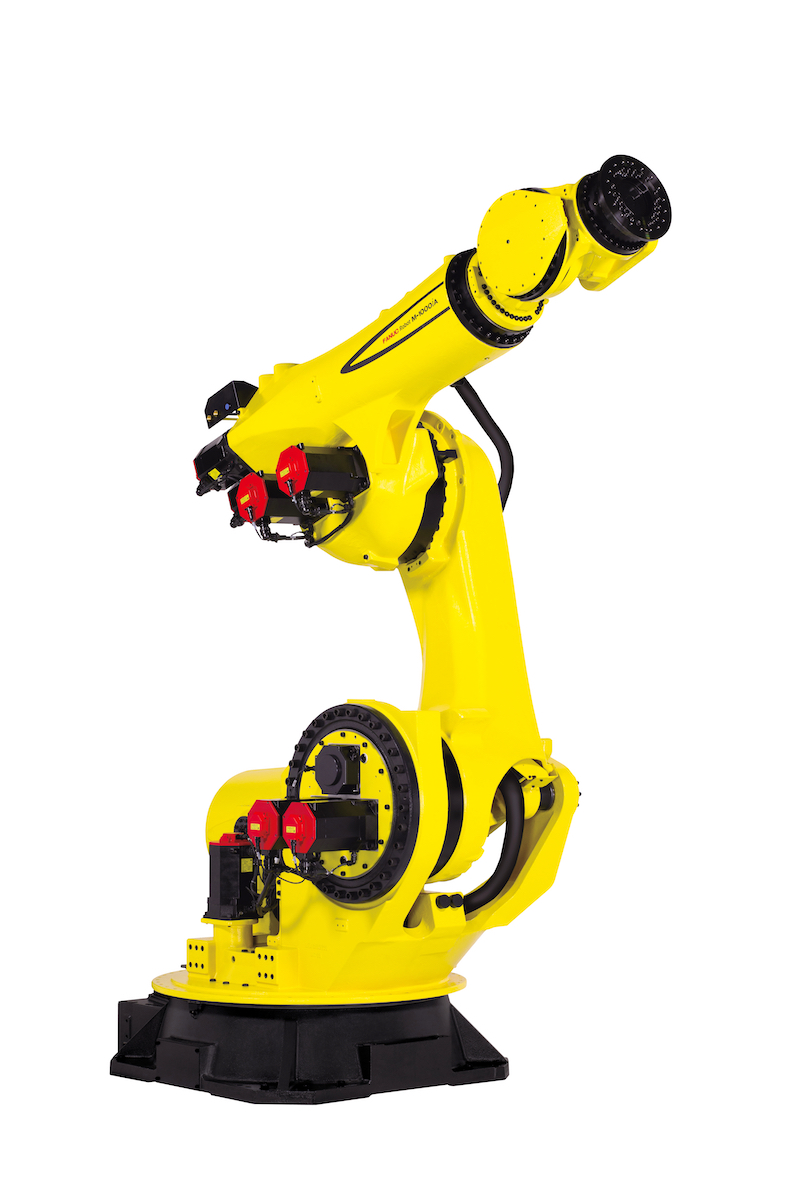
\includegraphics[width=0.3\textwidth]{Src/images/Robot.jpg}
	\caption{Indusrial robot arm}
\end{figure}

One of the main characteristics of any robot arm is the number of degrees of freedom(DoF), which is characterised by the set of motion axis parameters that the robot has.  It describes the freedom of movement of the robot arm or manipulator in its workspace.  The degrees of freedom of a robot arm are determined by the number of joints it has, each of which provides a specific axis of motion.

The degrees of freedom of the robot arm can be classified in one of two possible ways:
\begin{itemize}
    \item Linear Motion (Translational DoF)
    \item Rotational Motion (Rotational DoF)
\end{itemize}

Manipulator robots can be classified on the basis of their structure and movement capabilities. Each type is suitable for each application, rotating joints and often the preferred choice for tasks that involve reaching, grasping and positioning objects, as they allow for more flexible movement in a variety of directions. In scenarios where precise linear motion is required, such as assembly lines where components need to be moved in a straight line, prismatic couplings can be used. But it is not uncommon to use two types of motion in a robot design and they have become widespread.

There is no strict dependency on which type of robot arm should be used in a particular case. The choice of robot arm will still get the job done, but the right robot is necessary to maximise productivity and cost savings.




\subsection{Disadvantages of existing robotic arms}

There are various types of robot arms available in the market, some of them can be considered really small in size and suitable for the requirements.
Certain disadvantages exist that are often found in existing models of robot manipulators.





\begin{figure}[H]
	\centering
	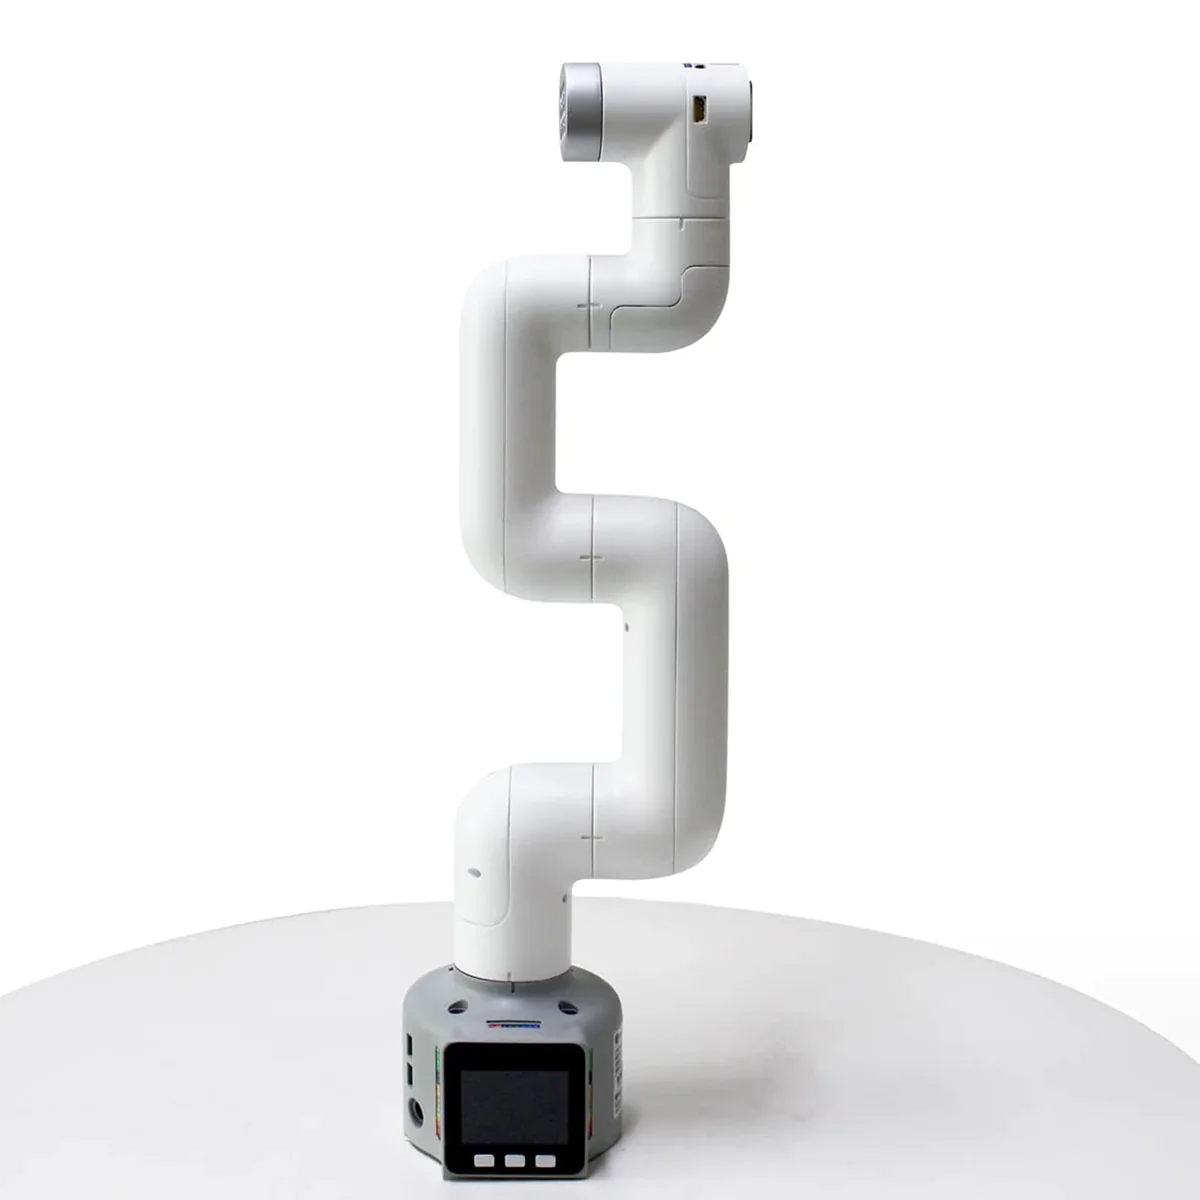
\includegraphics[width=0.4\textwidth]{Src/images/myCobot.png}
	\caption{MyCobot 280}
    \label{mycobot1}
    
\end{figure}
One of the popular models that is available on the market and can be available is the \textbf{myCobot} model robot, shown in the picture \ref*{mycobot1}, as well as technical specifications of the robots represents in the table \ref*{tab:mycobot1}.


\begin{table}[H]
    \caption{Specifications MyCobot Robot Arm}\label{tab:mycobot1}
    \centering
    \begin{tabular}{|l|c|c|}
        \hline
        \textit{\textbf{Parameter ame}} & \multicolumn{1}{l|}{\textit{\textbf{Value}}} & \multicolumn{1}{l|}{\textit{\textbf{Units}}} \\ \hline
        DOF                  & 6     & -     \\ \hline
        Payload              & 0.25  & kg    \\ \hline
        Weight               & 0.8   & kg    \\ \hline
        PRepeatability & ± 0.5 & mm    \\ \hline
        Power Voltage        & DC 12 & V     \\ \hline
        Power Current        & 5     & A     \\ \hline
        Gear type            & -     & Steel \\ \hline
        Shell                & -     & Metal \\ \hline
        Max. reach           & 280     & mm \\ \hline
        Cost                & 800    & Euro \\ \hline
        \end{tabular}
 \end{table}

 


 In most cases, one of the main factors in this type of robot is the use of more low-cost actuators that drive the robot's axis. This may be the use of more low-cost gearboxes and motors that greatly reduce the cost of the entire robot, but the lifetime of these systems is relatively short.

 In the process of testing the basic specifications that was explained that with not all the parameters that are presented in the table \ref*{mycobot1} data are not all reliable, the accuracy of movement is highly dependent on the load at the end of the 6 axis of the robot. Thus, the repeatability of the robot movement was not within \textbf{\pm 0.5 mm}, but could reach deviation around \textbf{ 5 mm}. As shown in figure \ref*{mycobot2} 

 \begin{figure}[H]
	\centering
	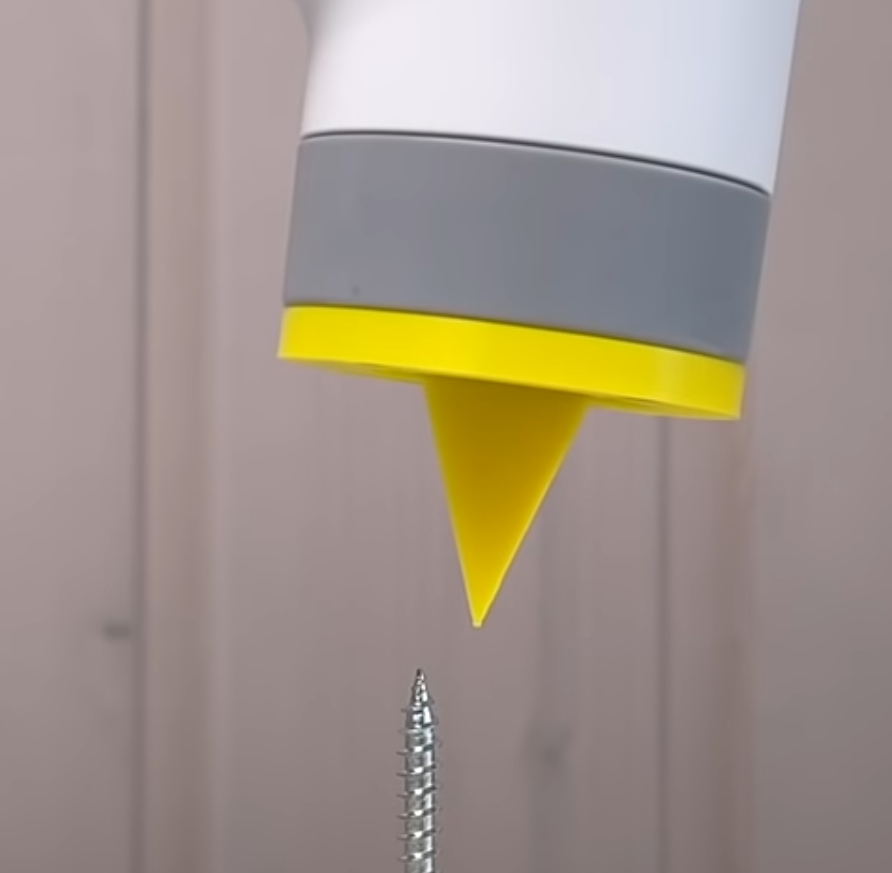
\includegraphics[width=0.4\textwidth]{Src/images/mycobot2.png}
	\caption{Robot repeatability measurement example}
    \label{mycobot2}
\end{figure}

In fact, the servomotors used in hobbyist versions of robotic manipulators, such as the one shown in figure \ref*{mycobot3}, are significantly less accurate and reliable than those used in their industrial counterparts. One of the main reasons for this is that these types of servos are typically designed with cost-effectiveness and basic functionality in mind, rather than high accuracy or durability. This can lead to inconsistent performance, frequent failures and a shorter overall life.


\begin{figure}[H]
	\centering
	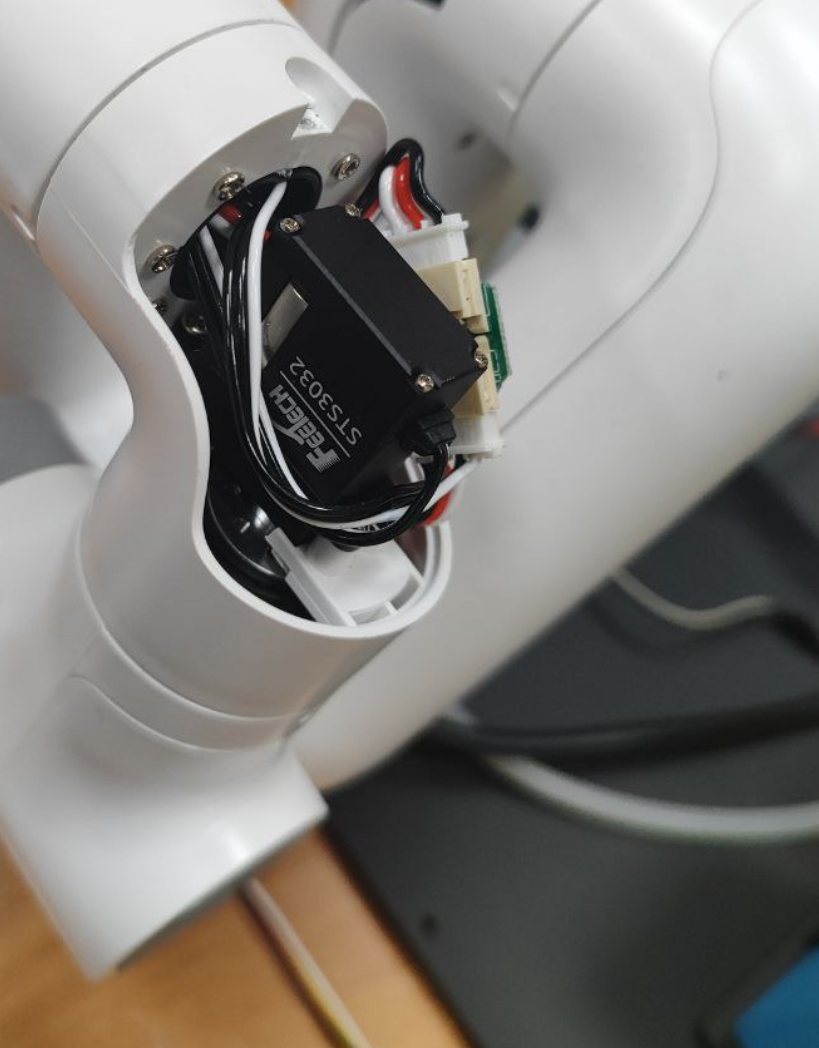
\includegraphics[width=0.4\textwidth]{Src/images/mycobot3.png}
	\caption{Hobbyist Servo Motor}
    \label{mycobot3}
\end{figure}


In addition, the lightweight construction of these servomotors can make them more susceptible to physical impact and other environmental factors. This lack of robustness often results in frequent maintenance, which can lead to increased downtime and reduced productivity.

Hobbyist servomotors often have less sophisticated control systems, which may not provide the advanced features required for precise control in complex applications. 

 \begin{figure}[H]
	\centering
	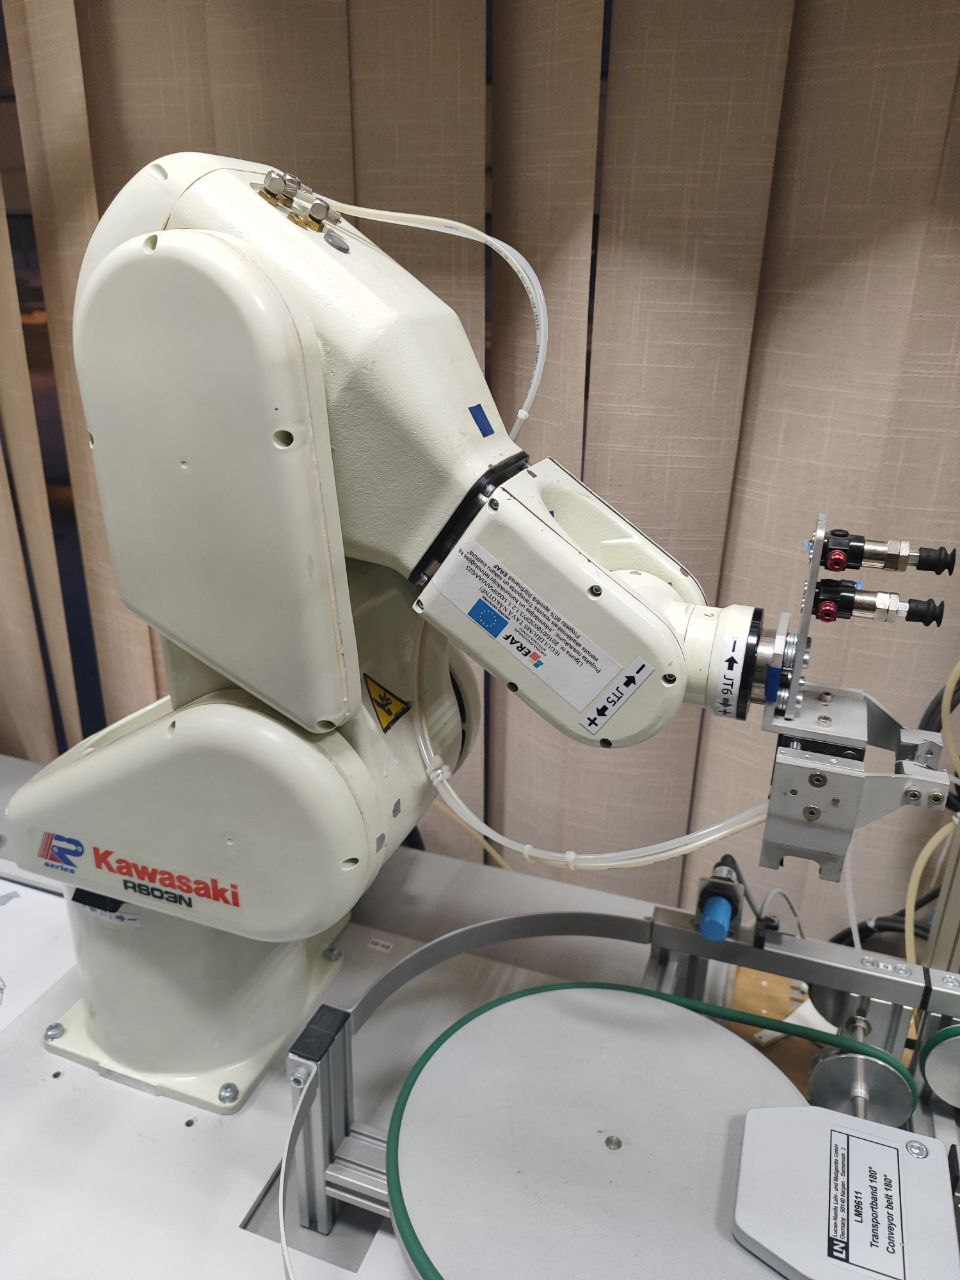
\includegraphics[width=0.6\textwidth]{Src/images/FS03N.jpg}
	\caption{Kawasaki FS03N}
    \label{Kawasaki1}
\end{figure}

\begin{table}[H]
    \caption{Specifications Kawasaki Robot Arm FS03N}\label{tab:Kawasaki1}
    \centering
    \begin{tabular}{|l|c|c|}
        \hline
        \textit{\textbf{Parameter ame}} & \multicolumn{1}{l|}{\textit{\textbf{Value}}} & \multicolumn{1}{l|}{\textit{\textbf{Units}}} \\ \hline
        DOF                  & 6     & -     \\ \hline
        Payload              & 3 & kg    \\ \hline
        Weight               & 20   & kg    \\ \hline
        Repeatability        & ± 0.02 & mm    \\ \hline
        Power Voltage        & AC 230 & V     \\ \hline
        Max Power Current    & 9    & A     \\ \hline
        Gear type            & -     & Steel \\ \hline
        Shell                & -     & Aluminium \\ \hline
        Max. reach           & 620     & mm \\ \hline
        Cost                & 12 000     & Euro \\ \hline
        \end{tabular}
 \end{table}

 
\begin{figure}[H]
	\centering
	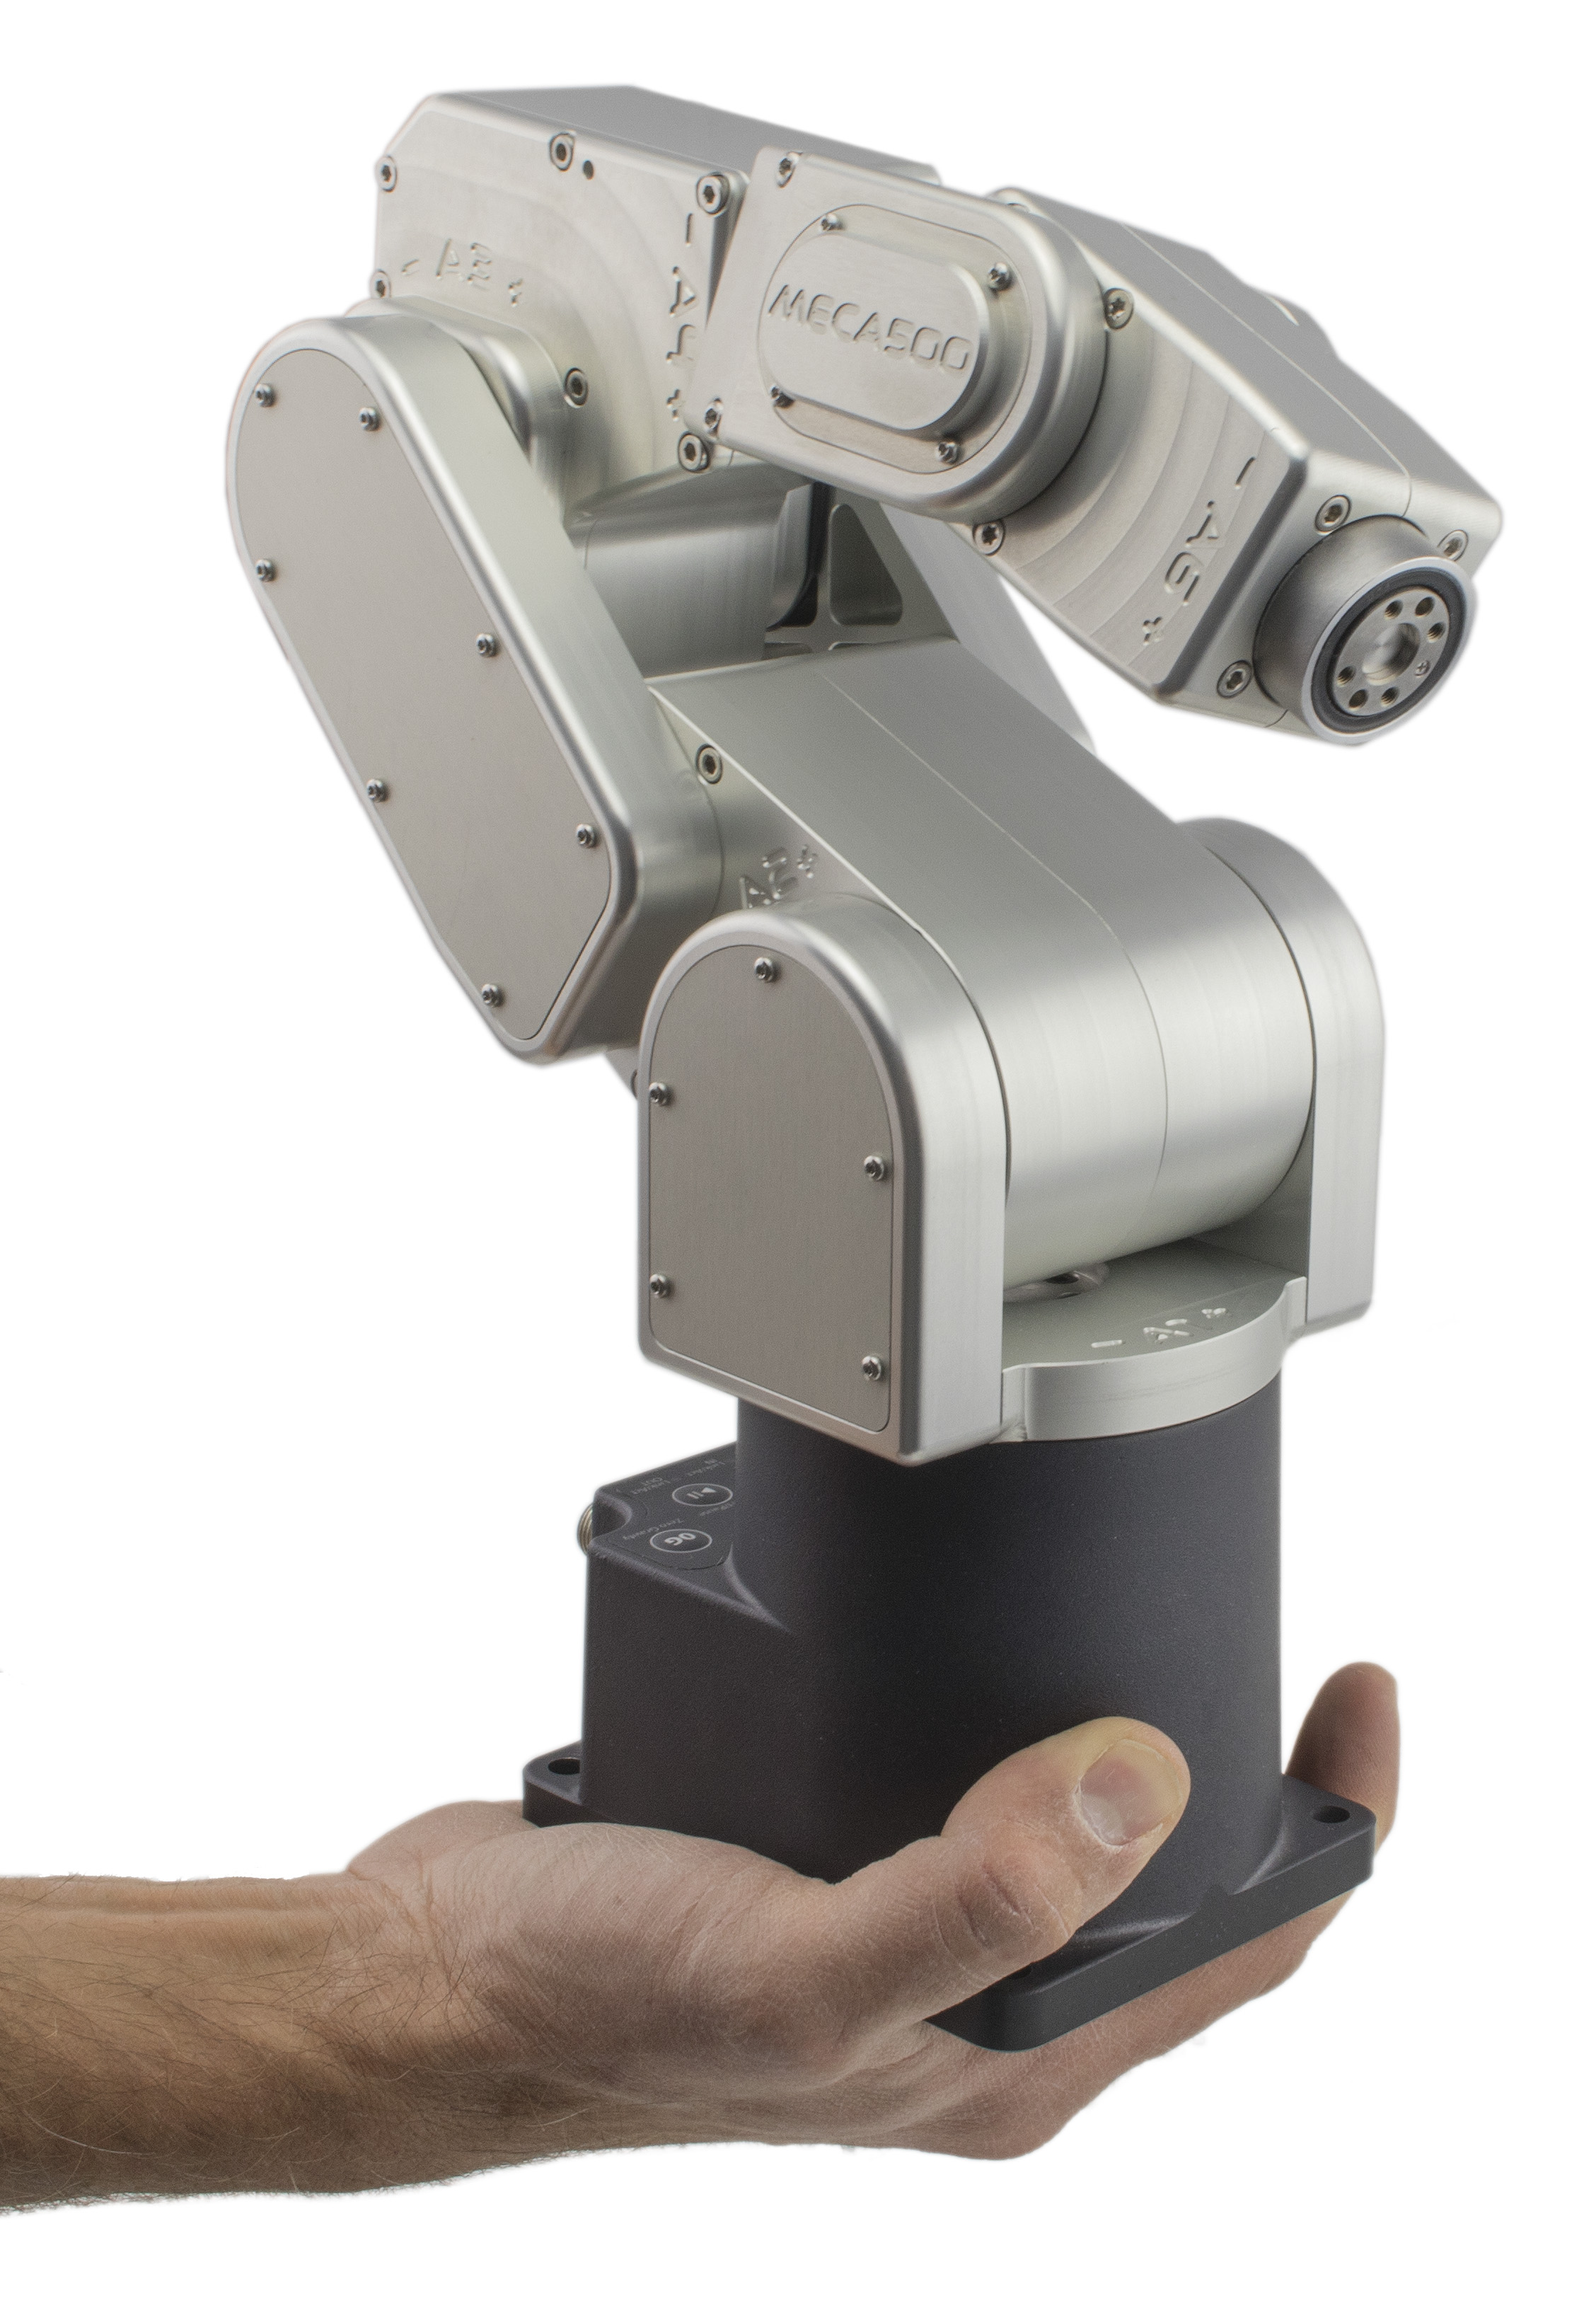
\includegraphics[width=0.4\textwidth]{Src/images/Meca500.jpg}
	\caption{Meca 500}
    \label{Meca1}
\end{figure}

\begin{table}[H]
    \caption{Specifications for Meca 500 Robot Arm}\label{tab:Meca1}
    \centering
    \begin{tabular}{|l|c|c|}
        \hline
        \textit{\textbf{Parameter ame}} & \multicolumn{1}{l|}{\textit{\textbf{Value}}} & \multicolumn{1}{l|}{\textit{\textbf{Units}}} \\ \hline
        DOF                  & 6     & -     \\ \hline
        Payload              & 0.5 & kg    \\ \hline
        Weight               & 4.5   & kg    \\ \hline
        PRepeatability & ± 0.005 & mm    \\ \hline
        Power Voltage        & DC 24 & V     \\ \hline
        Max Power Current        & 9    & A     \\ \hline
        Gear type            & -     & Steel \\ \hline
        Shell                & -     & Aluminium \\ \hline
        Max. reach           & 330     & mm \\ \hline
        Cost                & 12 000     & Euro \\ \hline
        \end{tabular}
 \end{table}

\subsection{Rationale for creating a miniature robotic manipulator}
Nowadays the use of mini robot manipulators in modern production is rare and most of any small works are created manually or it is necessary to create machines for a specific task, which takes more time to develop on a more universal basis. And the use of human resources is a human factor and quality is reduced in pursuit of quantity.

The problem can be solved by creating a new robot manipulator that will be suitable for interaction with small objects, as well as more cost-effective in the process of exploitation. 

\subsection{Сoncept of systems development}
\input{Src/chapters/Сoncept.tex}

%%%%%%%%%%%%%%%%%%%%%%%%%%%%%%%%%%%%%%%%%%%%%%%%%%%%%%%%%%%%%%%%%%%%%%%%%%%%%%%%%%%%%%%5
\section{Technical parameters of minirobot}
\subsection{Brief information about the robot arm} 

This chapter will provide a short description of the development of the minirobot control system.

The comparative characteristics of existing robot types are shown in the table \ref*{tab:robot_crt}

\begin{table}[H]
    \caption{Various types of robots and their characteristics}\label{tab:robot_crt}
    \centering
    \begin{tabular}{|l|c|c|c|}
    \hline
    \multicolumn{1}{|c|}{} & Speed                                & Accuracy                             & DoF                                      \\ \hline
    Robot Arm              & Low                                  & Middle                               & {\color[HTML]{FE0000} \textbf{High (6)}} \\ \hline
    Scara                  & Middle                               & {\color[HTML]{FE0000} \textbf{High}} & Middle (4)                               \\ \hline
    Delta                  & {\color[HTML]{FE0000} \textbf{High}} & Low                                  & Middle (4)                               \\ \hline
    \end{tabular}
 \end{table}


 For the implementation of the robot control system was chosen "Robot manipulator" because of the high degree of mobility of this type of robot, which contribute to a more convenient movement of objects in space.
%%%%%%%%%%%%%%%%%%%%%%%%%%%%%%%%%%%%%%%%%%%%%%%%%%%%%%%%%%%%%%%%%%%%%%%%%%%%%%%%%%%%%%%
\subsection{Industrial minirobot arm functions}  
\subsection{Industrial minirobot arm modes}


\section{Mechanical designs of minirobot arm}

\section{Functions and modes of operation of the minirobot control system }

\section{Development of the structural scheme of the minirobot control system}

\section{Development of functional and circuit diagrams of the minirobot control system}


\section{Development of algorithms and control programmes for the minirobot control system}


\section{Testing of the minirobot control system }

% \include{appendix.tex} %TODO
% \end{document}
